\documentclass{yThesis2}


% (*) Preparing figures:
% - dla linii 'lw 2' czyli grubosc 2, a dla error bars mozna zostawic domyslnie czyli (lw 1)
% - set terminal postscript eps enhanced color
% - najbardziej rozroznialne style: lt 1, 2, 3, etc. (do ustawienia stylu wystarczy 'lt x lw y' to ustawi kolor, rodzaj linii i grubosc
% - It looks that the best idea is to keep scaling=1.0 in latex all the time and then change the size in gnuplot only (e.g., set size 0.8, 0.8 in gnuplot). In this way all graphs have the same font size. Having this, one can produce figures of different sizes and font in all of them will be the same.
% - wszystkie skrypty do rozprawy beda mialy "\_thesis.plt" w koncowce nazwy


% this packages are for short citations in Latex
%\usepackage{dialogue}
%\usepackage{authordate1-4}
\usepackage{times}
\usepackage{setspace}
\usepackage[latin1]{inputenc}
\usepackage[UKenglish]{babel}
\usepackage{amsmath}
\usepackage{amsthm}
\usepackage{amssymb}
\usepackage{tabularx}
\usepackage{booktabs}
\usepackage{multirow}
\usepackage{subfigure}
\usepackage{verbatim}
\usepackage{float}
\usepackage{listings}
% to get the bibliography in the toc
\usepackage[nottoc,notlot,notlof,chapter]{tocbibind}
\usepackage{rotating}
\usepackage{titlesec}
\usepackage{url}
\usepackage{fancyhdr}
\usepackage{rst}
\usepackage{textcomp}
%\usepackage[greek,british]{babel}

%\usepackage{algorithms}
% \citet{jon90} ) Jones et al. (1990)
% \citet[chap.~2]{jon90} ) Jones et al. (1990, chap. 2)
% \citep{jon90} ) (Jones et al., 1990)
% \citep[chap.~2]{jon90} ) (Jones et al., 1990, chap. 2)
% \citep[see][]{jon90} ) (see Jones et al., 1990)
% \citep[see][chap.~2]{jon90} ) (see Jones et al., 1990, chap. 2)
% \citet*{jon90} ) Jones, Baker, and Williams (1990)
% \citep*{jon90} ) (Jones, Baker, and Williams, 1990)
% \citet{jon90,jam91} ) Jones et al. (1990); James et al. (1991)
% \citep{jon90,jam91} ) (Jones et al., 1990; James et al. 1991)
% \citep{jon90,jon91} ) (Jones et al., 1990, 1991)
% \citep{jon90a,jon90b} ) (Jones et al., 1990a,b)
\usepackage{natbib}
%\usepackage{makeidx}
%%index is better than makeindex as you can have more than one running
%%index file per document... this way, the author index is managed
%%separately
\usepackage{index}
%\usepackage{hyperref}
\usepackage[breaklinks=true]{hyperref}
\usepackage{qtree}
% The algorithm packages have to be after hyperref.
\usepackage{algorithm, algorithmic}
\usepackage{xspace, float, graphicx, pstricks}
\usepackage{wrapfig}
\usepackage[intoc,refpage]{nomencl} %refeq
\usepackage{longtable}
\usepackage{lscape}
\usepackage{slashbox}
%\usepackage{xfrac}
\makenomenclature

\usepackage{color}
\definecolor{javared}{rgb}{0.6,0,0} % for strings
\definecolor{javagreen}{rgb}{0.25,0.5,0.35} % comments
\definecolor{javapurple}{rgb}{0.5,0,0.35} % keywords
\definecolor{javadocblue}{rgb}{0.25,0.35,0.75} % javadoc
 
\lstset{language=Java,
basicstyle=\ttfamily,
keywordstyle=\color{javapurple}\bfseries,
stringstyle=\color{javared},
commentstyle=\color{javagreen},
morecomment=[s][\color{javadocblue}]{/**}{*/},
%numbers=left,
numberstyle=\tiny\color{black},
stepnumber=2,
numbersep=10pt,
tabsize=4,
showspaces=false,
showstringspaces=false}


\hypersetup{
   pdftitle = {New Strategies for Automated Random Testing},
   pdfsubject = {Ph.D. Thesis, The University of York},
   pdfkeywords = {phd, thesis, york, university, automated, random testing, YETI, software testing},
   pdfauthor = {\textcopyright\ \today\ Mian\'{s}},
   %pdfcreator = {\LaTeX\ with Emacs},
}


\setlength{\bibsep}{0pt}
\bibpunct[:]{(}{)}{;}{a}{}{,} % to format the way references are formatted inside the text
\renewcommand{\arraystretch}{1.17} % line spacing in tables
\setlength\tabcolsep{8pt} % column formatting in tables
\setcounter{tocdepth}{3} % how far the embedding goes in your TOC


\makeindex
%so natbib generates the author index
\citeindextrue
%so the author index is in an external citation file
%generate with:
%sed -e 's/{{\([^}]*\)}/{\1/g' main.adx > /tmp/main.adx; makeindex -s main.ist -o main.and /tmp/main.adx
\newindex{idx}{idx}{ind}{Index}
\newindex{aut}{adx}{and}{Citation Index}
\renewcommand{\citeindextype}{aut}


%%mark the things to do...
%\usepackage{color}
%\definecolor{Orange}{rgb}{1,0.5,0}
%\newcommand{\todo}[1]{\textsf{\textbf{\textcolor{Orange}{TODO [[#1]]}}}}
% Command for inserting a todo item
\usepackage{todonotes}
\reversemarginpar
\newcommand{\globaltodo}[1]{\addcontentsline{tdo}{todo}{Global: \protect{#1}}}
%\renewcommand{\todo}[1]{\todo[left]{#1}}
%%TODO%%
% (1) Type this: \listoftodos to generate a list of global TODOs
% (2) Each global TODO can be added in this way: \globaltodo{write here that to do}


% One of this too can be chosen.
%\usepackage[Bjornstrup]{fncychap}
\usepackage[Sonny]{fncychap}


\linespread{1.5}


% \makeglossary


\newtheorem{defin}{Definition}
\newtheorem{lemma}{Lemma}
\newtheorem{theor}{Theorem}


\title{New Strategies for\\[0.4cm]Automated Random Testing}
%\subtitle{Resources from Multilingual\\ Corpora and their
%Exploitation}
\author{Mian Asbat Ahmad}
\authoremail{mian.ahmad@york.ac.uk}
\dept{Department of Computer Science}
\submitdate{\today}


\begin{document}


% York reg 2.7.3 section l requires numbering from title page so \frontmatter can not be used.
% \onehalfspacing % looks better than double spacing, but \onehalfspacing is equivalent to \linespread{1.3}
% \mainmatter % is is necessary when the book class is used.


% % %%%%%%%%%%%%%%%%%%%%%% START HERE %%%%%%%%%%%%%%%%%%%%%%%%%%%%%%%%%%

\pagenumbering{roman}

% (1) The title page.
\titlePage

% (2) \correctionsPage

% (3) Abstract
\yabstract{This is the abstract text with the formula $v_L(t)=\int^t_{-\infty}
\frac{di_L}{dt}$. This paper describes the computation of feature
point correspondences using the spectra of a Hermitian property
matrix. Firstly, a complex Laplacian (Hermitian) matrix is
constructed from the Gaussian-weighted distances and the difference
of SIFT angles between each pair of points in the two images to be
matched. Matches are computed by comparing the complex eigenvectors
of the Hermitian property matrices for the two point sets acquired
from the two images. Secondly, we embed the complex modal structure
within Carcassoni's iterative alignment method to render it more
robust to rotation. Our method has been evaluated on both synthetic
and real-world data.
}

% (4) Table of contents, list of tables, list of figures.
\contents

% (5) Preface, if any, would go here.
%\preface{\input{preface}}

% (6) Acknowledgement
\acknowledgement{\input{Acknowledgements}}

% (7) Declaration and published work.
\declaration{\input{Declaration}
%\paragraph{Publications}

%\begin{figure}[b]
%\begin{center}
%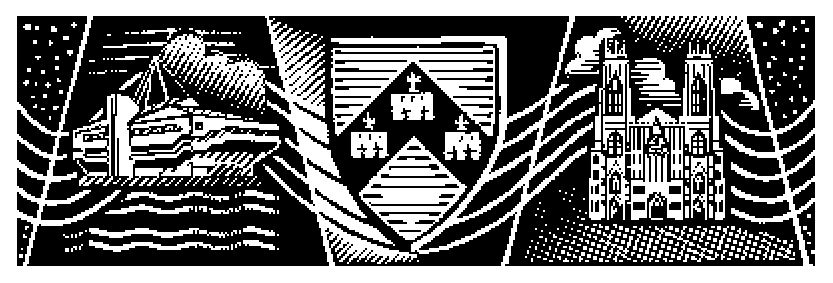
\includegraphics [width=7cm] {Woodcuts/univwoodcut}
%\end{center}
%\end{figure}
}

\newpage
\newpage
\newpage

\pagenumbering{arabic}

% (1.1) to whom: it goes to the second page immediately after the title page
\dedication{I feel it a great honour to dedicate my PhD thesis to my beloved parents for their significant contribution in achieving the goal of academic excellence reflected in my dissertation.
}

%%inroduction
\ychapter{Introduction}{Introduction}{

Today, the primary focus of software companies is to achieve high quality. These companies spend an estimated thirty to ninety percent of the total software development cost on testing \ref{Beizer1990}, \ref{Standards2002}. 

Software testing is the process of executing a software with specific test data followed by evaluation of the results to check whether it is working according to its specification or not \ref{Sommerville2006}.
% check here if we can replace specification with oracle or not.
The test passes if the output complies to its specification and fails otherwise. The success of testing correlates with the number of failures found in the Software Under Test (SUT): a test is more successful if it finds more faults.

It is interesting that program testing is used to show the presence of bugs, rather than absence of bugs [6]. Therefore the SUT that passes all the tests without returning a single failure does not guarantee that there is no fault. The testing process increases however the reliability and confidence of both the developers and the users in the tested product [7] [8] [9].

Random testing is a black-box testing technique in which the SUT is executed against ran- domly selected test data. Test results obtained are compared either against the oracle defined, using SUT specifications in the form of assertions or exceptions defined by the programming language. The rapid increase in software development in today?s modern world prompts the need for automated testing to ensure high quality. The generation of random test data is com- paratively cheap and does not require too much intellectual and computation efforts [10] [11]. It is for this reason that various researchers have recommended this strategy for incorporation in automatic testing tools [12]. YETI [13] [14], AutoTest [15] [16], QuickCheck [17], Randoop [18], JArtage [19] are a few of the most common tools based on random strategy.

\section{Problem Description}
\subsection{Test input data is decisive}
\subsection{Selecting Fault finding input is challenging}

\section{Our Goals}

\section{Contributions}
\subsection{Dirt Spot Sweeping Random Strategy}
\subsection{Automated Discovery of Failure Domain}
\subsection{Directed Random Plus Strategy}

\section{Thesis Outline}}


%%literature review
\ychapter{Literature Review}{Literature
Review\label{CHAP:FIELDREV}}{
\section{Software Testing}
\subsection{Categories of Software Testing}
\subsubsection{Black-box Testing}
\subsubsection{White-box Testing}
\subsection{Manual Testing}
\subsection{Automated Testing}
\subsubsection{Random Testing}
\subsubsection{Exhaustive Testing}

\section{Automated Random Testing}
\subsection{Test Data Generation}
\subsection{Test Execution}
\subsection{Test Oracle}
\subsection{Test Report}

\section{Variations is Random Testing}
\subsection{Adaptive Random Testing}
\subsection{Mirror Adaptive Random Testing}
\subsection{Directed Automated Random Testing}
\subsection{Quasi Random Testing}
\subsection{Monti Carlo Random Testing}
\subsection{Good Random Testing}
\subsection{Feedback-directed Random Testing}
\subsection{Adaptive Random Testing for Object-Oriented}
\subsection{Restricted Random Testing}

\section{Automated Random Testing Tools}
\subsection{JCrasher}
\subsection{JArtage}
\subsection{Eclat}
\subsection{JTest}
\subsection{QuickCheck}
\subsection{AgitarOne}
\subsection{Autotost}
\subsection{TestEra}
\subsection{Korat}
\subsection{RANDOOP}
\subsection{YETI}


\section{Conclusion}


}%{\input{FieldReview}}

%% The chapter on plan-based reward shaping.
%\ychapter{Design OR Title of the Paper}{Design OR Title of the
%Paper\label{CHAP:STRIPS}}{\input{STRIPS_Rshaping}}

%% The chapter on r-s from mixed resolution function approximation
\ychapter{Dirt Spot Sweeping Random Strategy}{Dirt Spot Sweeping Random Strategy\label{CHAP:DSSR}}{\input{DirtSpotSweepingRandomStrategy}}%{\input{TwoAbstractionsInCMAC}}

%% The chapter on the Reward Shaping Analysis in model-free RL
%\ychapter{Extraction of Multilingual Synsets from Aligned
%Corpora}{Extraction of Multilingual Synsets from Aligned
%Corpora\label{CHAP:RSANALYSIS}}{\input{Rshaping_Analysis}}

\ychapter{Automated Discovery of Failure Domain Strategy}{Automated Discovery of Failure Domain Strategy\label{CHAP:ADFD}}{\input{AutomatedDiscoveryOfFailureDomainStrategy}}

\ychapter{Directed Random Plus Strategy}{Directed Random Plus Strategy\label{CHAP:DRPS}}{\input{DirectedRandomPlusStrategy}}

%% The chapter on the use of knowledge-based admissible models in PAC-MDP learning
%\ychapter{Evaluation on Artificial Corpus}{Evaluation on Artificial
%Corpus\label{CHAP:PACMDPADMISSMODELS}}{\input{PACMDP_Admissible_Models}}

%% The chapter on the Analysis of Eligibility Traces
%\ychapter{Analysis of Exploration with Eligibility Traces}{Analysis of Exploration with Eligibility Traces\label{CHAP:ELTRACES}}{\input{Eligibility_Traces_Analysis}}

%%conclusion
\ychapter{Conclusion}{Conclusion\label{CHAP:CONCLUSION}}{\input{Conclusion}}


% %%%%%%%%%%%%%%%%%%%%% APPENDIX ETC %%%%%%%%%%%%%%%%%%%%%%%%%%%%%%%%%%%%

%\begin{appendix}
%\addcontentsline{toc}{chapter}{Appendices}
%--  \input{desertquestionnaire}
%--  \input{restoquestionnaire}
%--  \input{desertgraph}
%\end{appendix}


% (*) Definitions before glossary. Definitions can be easily done with the nomencl package (used in the thesis template from Cambridge).

% (*) Glossary before references.
% %  \input{}
% %   \yorkGlossary  Terms that require explanation
% %                     shall be defined in a glossary, which shall
% %                     include a key to any abbreviations used. For
% %                     an abbreviation not in common use, the term
% %                     shall be given in full at the first instance
% %                     followed by the abbreviation in brackets.
%   \input{Cglossary}

%\backmatter
%bibtex setup and path names

%latex get crazy if we don't disconnect natbib citeindex
\citeindexfalse
\renewcommand{\bibname}{References}
% I am changing the original bibliography style from newapa to bibtex by commenting the following line and adding another asbat.
%\bibliographystyle{newapa}
\bibliographystyle{plain}
%\bibliography{../../mybib}
\bibliography{mybib}

%\yorkBib{}


% index.bat has to be executed to process index files.
\yorkIndex
\yorkCiteIndex
\yorkNomIndex

\begin{figure}[b]
 \begin{center}
 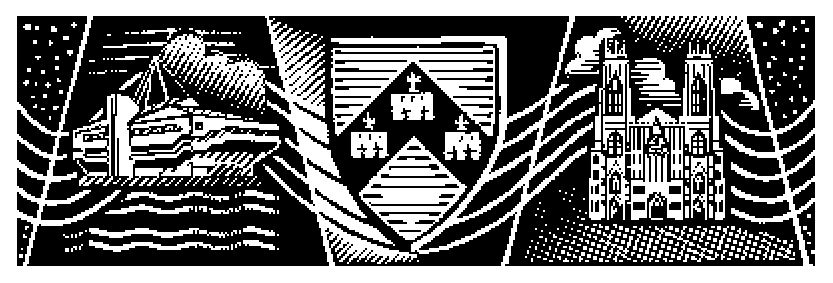
\includegraphics [width=7cm] {Woodcuts/univwoodcut}
\end{center}
\end{figure}

%\ylastpage{
%\begin{picture}(0.0,0.0)
%  \put(80,-550){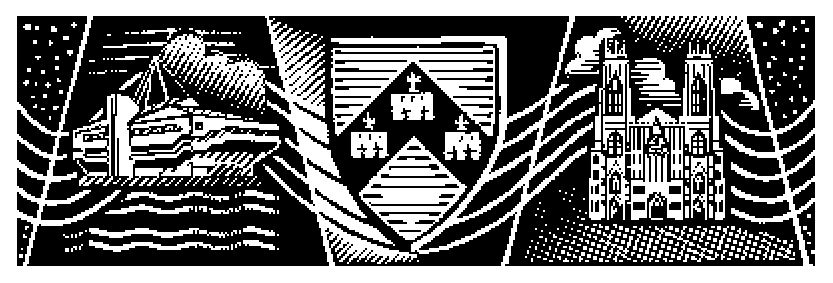
\includegraphics[width=7cm]{Woodcuts/univwoodcut}}
%\end{picture}
%}


%\include{ThesisTodo}



\end{document}
